\documentclass[11pt,a4paper]{article}
\usepackage[a4paper,margin=2cm,headheight=16pt,headsep=5mm]{geometry}
\usepackage[T1]{fontenc}
\usepackage{newtxtext,newtxmath}
\usepackage{graphicx,booktabs,tabularx,xcolor,enumitem,microtype}
\usepackage[font=small,skip=3pt]{caption}
\usepackage[hidelinks]{hyperref}
\usepackage{titlesec,float,fancyhdr}
\usepackage[most]{tcolorbox}
\usetikzlibrary{arrows.meta,positioning}

\graphicspath{{figures/}}
\titleformat{\section}{\large\bfseries}{\thesection}{0.6em}{}
\titlespacing*{\section}{0pt}{7pt}{2pt}
\setlist{nosep,leftmargin=1.3em}
\setlength{\parindent}{0pt}
\setlength{\parskip}{3pt}
\setlength{\textfloatsep}{8pt}
\setlength{\intextsep}{6pt}
\newcommand{\ocr}[1]{\texttt{#1}}
\newcommand{\run}[1]{\textbf{#1}\enspace}

\pagestyle{fancy}
\fancyhf{}
\fancyhead[R]{\small\textsc{OCR + NLP pipeline}}
\fancyfoot[C]{\small\thepage}
\renewcommand{\headrulewidth}{0.4pt}

\begin{document}

\begin{center}
{\LARGE\bfseries Classifying superimposed image text}\\[3mm]
{\large Ofir Yeshurun}
\end{center}

\begin{tcolorbox}[colback=black!5,colframe=black!5,arc=1mm,left=2mm,right=2mm,top=1mm,bottom=1mm]
\textbf{Summary.} A pipeline classifying images as \ocr{alcohol} or \ocr{non\_alcohol} based on superimposed text. Images are contrast-enhanced with LAB-CLAHE and parsed by PaddleOCR (PP-OCRv6 small); if OCR confidence drops below 0.9, OCR re-runs on a horizontally mirrored image. Extracted text is then cleaned and scored with a character $n$-gram TF-IDF logistic regression classifier.
\end{tcolorbox}

\section{Data exploration}
For the analysis, I annotated 60 training images (30 per class) to record their superimposed text.
\begin{itemize}
\item The dataset is balanced, with 550 images per class. It is not redistributed with the code.
\item Each superimposed text holds one key term (alcoholic or not), often inside a short sentence (``Try event imported \emph{lager} premium'', Figure~\ref{fig:tricks}a).
\item Some alcohol terms are drink names (Figure~\ref{fig:tricks}a); others are brand names only (Figure~\ref{fig:tricks}b).
\item Non-alcohol cases are near-domain: other beverages and cannabis-related terms (Figure~\ref{fig:tricks}c, d).
\item Both classes contain text distortions: mirroring, rotation, split characters, etc. (Figure~\ref{fig:tricks}b, e-h).
\item Text is placed either inside a solid bounding box (Figure~\ref{fig:tricks}a) or directly over the image (Figure~\ref{fig:tricks}b).
\item Some photos contain their own text, such as signs and labels (Figure~\ref{fig:tricks}i).
\end{itemize}

\begin{figure}[H]
\centering
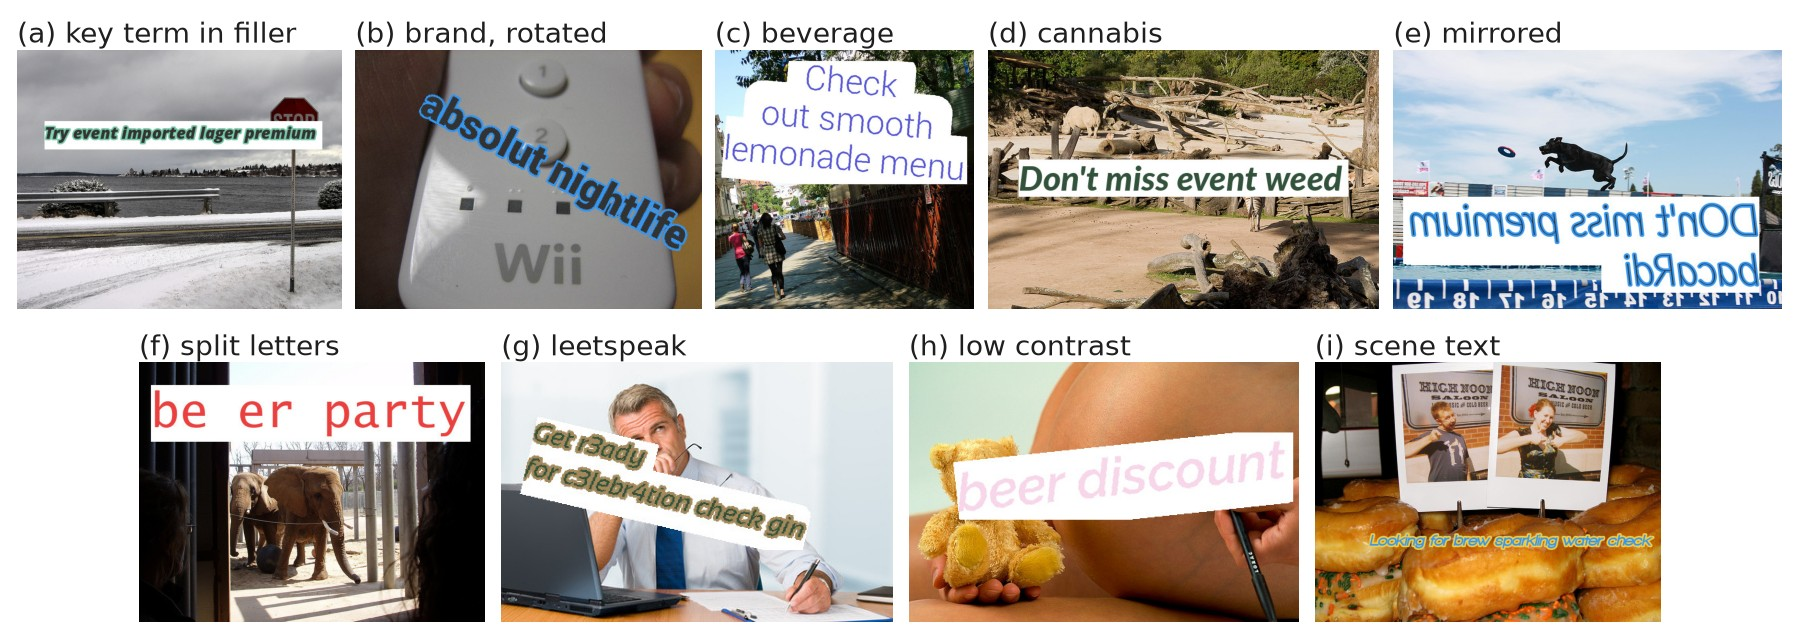
\includegraphics[width=\textwidth]{eda_trick_examples.jpg}
\caption{Train examples: (a, b, e-h) alcohol, (c, d, i) non-alcohol. (i) The superimposed text reads ``Looking for brew sparkling water check'', but the photo's sign says ``cold beer''.}
\label{fig:tricks}
\end{figure}

\section{Methodology}
\run{Assumptions.} Framing the classifier as a content-moderation filter, my main assumption was that a missed alcohol image is more harmful than a false positive, so throughout the project recall on alcohol was the primary metric.

\run{Protocol.} A stratified 70/15/15 split (seeded). Every choice was made by stratified 5-fold cross-validation. The test split was scored once, by the inference script (\texttt{scripts/inference.py}).

\run{Pipeline} (Figure~\ref{fig:pipeline}).

\begin{figure}[H]
\centering
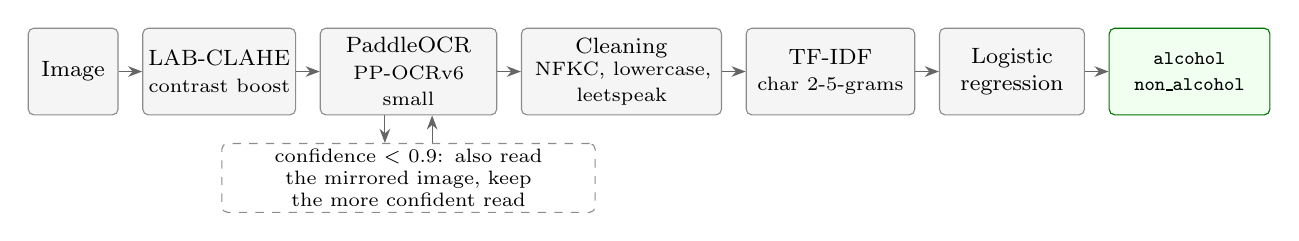
\begin{tikzpicture}[
  node distance=3mm,
  box/.style={draw=black!45, rounded corners=2pt, fill=black!4, align=center, font=\footnotesize, inner sep=2pt, minimum height=11mm, text width=#1},
  arr/.style={-{Stealth[length=1.8mm]}, black!60},
]
\node[box=10mm] (img) {Image};
\node[box=18mm, right=of img] (clahe) {LAB-CLAHE\\{\scriptsize contrast boost}};
\node[box=21mm, right=of clahe] (ocr) {PaddleOCR\\{\scriptsize PP-OCRv6 small}};
\node[box=24mm, right=of ocr] (clean) {Cleaning\\{\scriptsize NFKC, lowercase,\\leetspeak}};
\node[box=20mm, right=of clean] (tfidf) {TF-IDF\\{\scriptsize char 2-5-grams}};
\node[box=17mm, right=of tfidf] (lr) {Logistic\\regression};
\node[box=19mm, right=of lr, fill=green!6, draw=green!45!black] (out) {{\scriptsize\ocr{alcohol}}\\{\scriptsize\ocr{non\_alcohol}}};
\node[box=46mm, below=3.5mm of ocr, minimum height=7mm, dashed, fill=none, font=\scriptsize] (mir) {confidence $<$ 0.9: also read the mirrored image, keep the more confident read};
\draw[arr] (img) -- (clahe);
\draw[arr] (clahe) -- (ocr);
\draw[arr] (ocr) -- (clean);
\draw[arr] (clean) -- (tfidf);
\draw[arr] (tfidf) -- (lr);
\draw[arr] (lr) -- (out);
\draw[arr] ([xshift=-3mm]ocr.south) -- ([xshift=-3mm]mir.north);
\draw[arr] ([xshift=3mm]mir.north) -- ([xshift=3mm]ocr.south);
\end{tikzpicture}
\caption{The shipped pipeline.}
\label{fig:pipeline}
\end{figure}

\newpage
\section{Experiments}
\run{Choosing the OCR engine.} On the annotated sample, scored by \emph{key-term hit rate} (the share of images whose key term the OCR read), \texttt{PP-OCRv6-medium} led on raw images with 0.67, over \texttt{v6-small} (0.58) and \texttt{PP-OCRv5-mobile} (0.50).\\
Most missed cases were mirrored text, so I added a retry on the mirrored image when OCR confidence dropped below 0.9. This increased the hit rate to 0.87 (\texttt{v6-medium}) and 0.82 (\texttt{v6-small}), stable across several confidence thresholds.

\run{Rotated and faint text.} The same retry mechanism applied to rotations ($\pm$20$^\circ$) added no alcohol hits and more than doubled the extraction time per image. I tried several preprocessing methods to improve reads of faint text (CLAHE variants, top-hat and others); each improved a few images but worsened more of them. The exception was LAB-CLAHE: on v6-small it fixed a few alcohol images and broke none.
\vspace{0.5em}

\noindent\begin{minipage}[c]{0.52\textwidth}
\run{Classifiers.}
\begin{itemize}
\item \emph{v0, lexicon matching:} fuzzy matching against a domain-knowledge lexicon of alcohol terms, with an error margin that grows with term length.
\item \emph{v1, character 2-5-gram TF-IDF + logistic regression.} Error analysis showed that OCR mostly dropped characters, and short letter chunks survive that.
\item \emph{v2, frozen MiniLM embeddings + logistic regression.} Embeddings should carry knowledge to brands unseen in training.
\end{itemize}
v1 led on every OCR setup. v2 trailed, I assume because near-domain negatives (lemonade, espresso or CBD) sit close to alcohol in the embedding space. For v1 the OCR setups overlap. However, small + LAB-CLAHE had the highest recall at a quarter of medium's image processing time (Table~\ref{tab:ocr}).
\end{minipage}\hfill
\begin{minipage}[c]{0.45\textwidth}
\centering
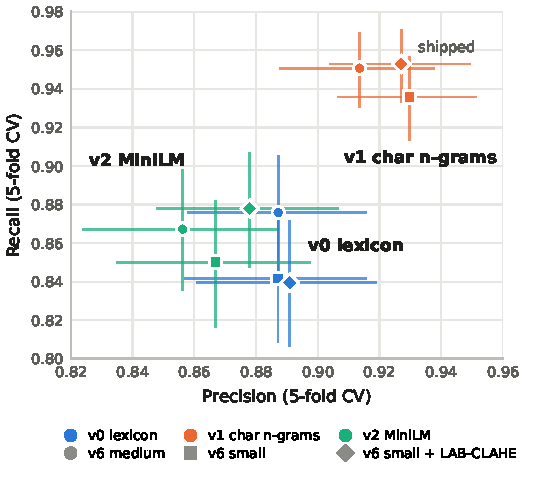
\includegraphics[width=\linewidth]{classifiers_cv.pdf}
\captionof{figure}{Recall vs precision with 95\% intervals, per classifier and OCR setup.}
\label{fig:models}
\end{minipage}

\begin{table}[H]
\centering\small
\caption{OCR engine trade-off, best setup per PP-OCRv6 engine.}
\label{tab:ocr}
\setlength{\tabcolsep}{4.5pt}
\begin{tabular}{lcccccc}
\toprule
OCR setup & Key-term hit* & Alcohol terms read* & Text found & Recall & Precision & s/img \\
\midrule
Medium, raw image & 0.867 & 28/30 & 98.4\% & 0.951 & 0.914 & 3.31 \\
Small + LAB CLAHE (shipped) & 0.850 & 25/30 & 97.1\% & \textbf{0.953} & \textbf{0.927} & \textbf{0.83} \\
\bottomrule
\end{tabular}

\vspace{1pt}{\footnotesize *On the annotated sample. Other columns: all train+val images; recall and precision are v1's CV scores.}
\end{table}

\section{Final performance}
\noindent\begin{minipage}[c]{0.56\textwidth}
\centering\small
\captionof{table}{Test split.}
\label{tab:test}
\begin{tabular}{lcc}
\toprule
 & Test, 165 images & CV, 935 images \\
\midrule
Recall & \textbf{0.916} [0.852, 0.973] & 0.953 [0.933, 0.971] \\
Precision & \textbf{0.916} [0.853, 0.974] & 0.927 [0.904, 0.949] \\
F1 & 0.916 [0.867, 0.956] & 0.940 [0.924, 0.955] \\
\bottomrule
\end{tabular}

\vspace{8pt}
\raggedright\normalsize
On test, recall and precision are both 0.916 (accuracy 0.915): fewer than one in ten alcohol images is missed, and fewer than one in ten non-alcohol images is wrongly flagged. Inference took 0.75\,s per image on CPU.
\end{minipage}\hfill
\begin{minipage}[c]{0.40\textwidth}
\centering
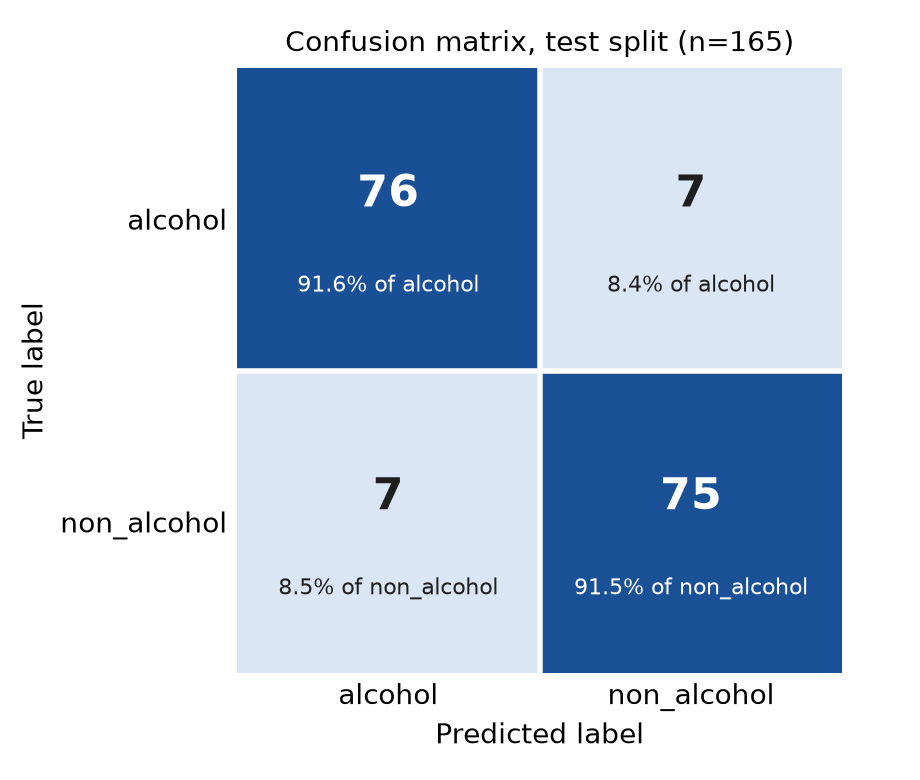
\includegraphics[width=\linewidth]{test_confusion_matrix.png}
\end{minipage}

\section{Failure cases and ideas for improvement}

\begin{figure}[H]
\centering
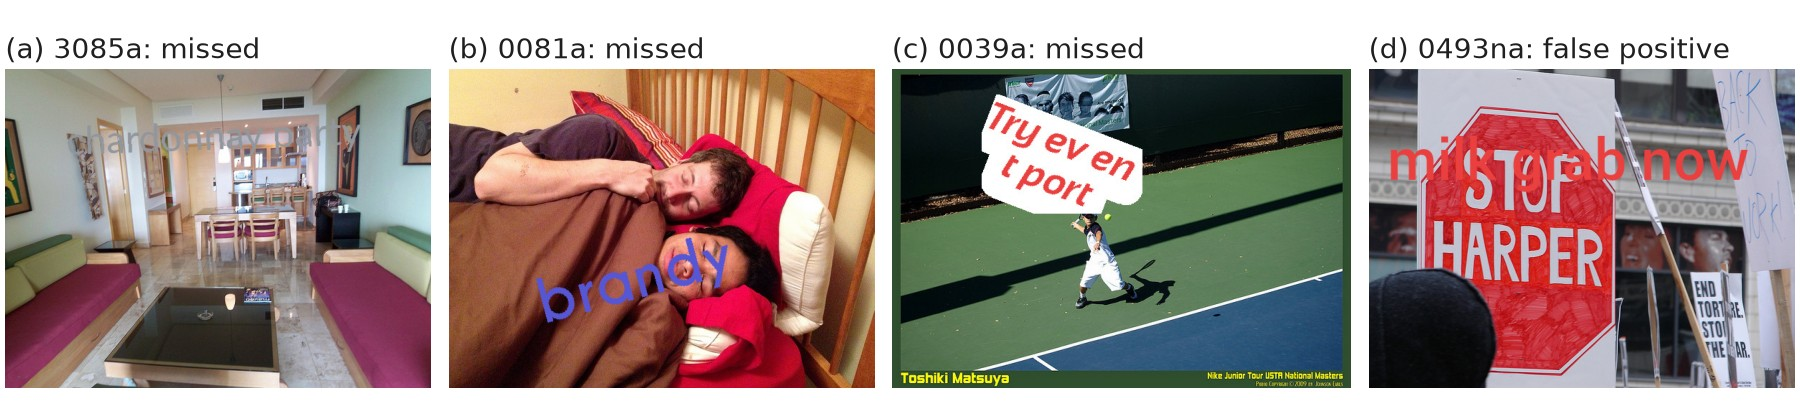
\includegraphics[width=\textwidth]{failure_test_cases.jpg}
\caption{Examples of test errors: (a)-(c) missed alcohol images, (d) a non-alcohol image flagged as alcohol (false positive).}
\label{fig:failures}
\end{figure}

\begin{table}[H]
\centering\small
\caption{What went wrong in each case, and the fix it points to.}
\label{tab:errors}
\begin{tabularx}{\textwidth}{@{}l >{\raggedright\arraybackslash}p{30mm} >{\raggedright\arraybackslash}X >{\raggedright\arraybackslash}X@{}}
\toprule
Case & OCR read & Likely reason & Suggested fix \\
\midrule
(a) 0.44 & \ocr{XsNAob16} & OCR missed the faint, semi-transparent text & An extra preprocessing retry on weak reads \\
(b) 0.48 & \ocr{Ybnpid} & Rotated text read weakly, so the mirror retry ran and its distorted read won & Keep the mirrored read only when it is clearly more confident \\
(c) 0.46 & \ocr{Tryeven tport ToshikiMatsuya Nike ...} & Split letters (``t port'') glued into one word; background text added noise & Re-segment split and glued fragments (\ocr{Tryeven tport} $\rightarrow$ \ocr{try event port}, \ocr{be er} $\rightarrow$ \ocr{beer}); down-weight scene text \\
(d) 0.53 & \ocr{STUPb now ... HARPER END ...} & ``milk'' lost (red text on a red sign); the sign's text drives the score & Down-weight scene text; try other preprocessing views \\
\bottomrule
\end{tabularx}
\end{table}

\end{document}
